\chapter{相关技术介绍}
\section{引言}
在自然语言处理研究领域中,基于神经网络的分布式表示(Distributional Representation)一般统称为词向量(Word Vector)、词嵌入(Word Embedding)或者分布式表示(Distributed Representation)~\upcite{DBLP:conf/nips/MikolovSCCD13}。神经网络词向量表示技术,是通过神经网络技术对:1)单词的语境,即上下文(Context);2)以及上下文与下一步的目标单词之间的关系(Next-Utterance Prediction),这两个主要的部分进行建模。
由于神经网络结构或各种组合较为灵活,这类方法的最大优势在于可以表示复杂的上下文语义(Complex Context)。历史上的方法主要是基于单词共现矩阵(Co-occurrence Matrix)的分布表示方法,最常用的上下文仅仅是利用了单词的顺序信息。单词的语义向量是通过给这个单词共现矩阵进行矩阵分解,例如奇异值分解(Singular Value Decomposition,SVD),潜在语义分析(Latent Semantic Analysis,LSA),也可以写成潜在语义索引(Latent Semantic Indexing,LSI)分解算法。其中对于SVD分解算法,第一个分解获得的矩阵就是我们模型输出的单词的词向量矩阵。然而,如果使用包含词序信息的~N-gram~作为上下文,当~$N$~增加时,N-gram 的所需要存储的单词序列总数会呈指数级增长,此时会遇到维数灾难问题(Curse of Dimensionality)\footnote{https://en.wikipedia.org/wiki/Curse\_of\_dimensionality}。这一瓶颈深深限制了~N-gram~模型的实际应用。而用神经网络替代表示~N-gram~的单词概率分布时,可以通过一些组合方式对~N~个词进行组合,其优点显而易见:神经网络语言模型所需要的参数数量仅以线性速度增长。有了这一优势,神经网络模型可以对更复杂的上下文进行建模,在从训练后的模型提取出来的词向量中包含更丰富的语义信息。

到目前为止,在语言模型的研究领域中,所应用到的神经网络模型主要包括: 传统前向传递神经网络(Feed Forward Neural Network, FFNN)、循环神经网络(Recurrent Neural Network, RNN)三种基本的建模方案。当然基于这些基本组件,我们还可以构造更复杂的模型结构,但是我们无法保证复杂模型一定在效率和精确度上优于简洁的模型结构。复杂的模型可以表征更复杂的本文语义信息,例如句子的依存关系结构或者句子的句法分析树结构,但是这样的效果不一定能保证模型的泛化性能(Generalization)会很好,因为日常聊天文本的语序是混乱的,很难找到学者良好定义的句子关系,所以也无法让模型从混乱的文本分布中学习到有效的句子结构,以提升模型的精度。最好的模型,显然是假设越弱越合适,因为针对复杂的网络文本数据,我们模型训练所需要的要求越弱,模型越容易收敛并获得我们想要的结果。模型假设越强,模型所需要的数据质量越高,实际稳定性就会降低,产生得不偿失的后果。

语言模型的历史发展
除此以外,针对在本论文所讨论的语言模型的大规模应用过程中所遇到的大词表问题,目前现有的主要解决方法主要可以分为以下三种种策略:单词拆分算法(Vocabulary Truncation)、采样估计模型(Sampling-based Approximation)和层次分解模型(Vocabulary Factorisation),我们会在接下来的章节陆续介绍。其中本论文重点是研究基于类别的多元分类模型(class-based hierarchical softmax, cHSM)和基于二叉树的二元分类模型(class-based hierarchical softmax,tHSM),这两种算法我们分别在下一章更详细讨论和介绍。

\section{语言模型}
在这一节中,我们将首先从语言模型提出的实际任务的形式化定义开始,以阐述语言模型的训练目标和实际应用场景~\upcite{DBLP:journals/tnn/ChienK16}。一个好的语言模型应当考虑对文本的两种特征进行建模:语法特征(Syntactics)和语义特征(Semantics)。为了保证语法的正确性,我们往往只需要考虑生成的单词的前面的上下文(Previous Context),这也就意味着语法特性往往只对局部特征(Local Representation)进行建模。而语义特征的一致性则复杂了许多,它意味着我们需要考虑更大、更完善的上下文信息乃至整个文档语料,来获取正确的全局语义(Global Context)而不仅仅是局部语义信息(Local Context)。


具体地来说,给定一个包含$T$个单词的序列:$w_1,w_2,\cdots,w_T$,这个序列的对数概率(Log-probability),即描述该序列作为一个合理且合法的句子的流畅性(Fluency)概率和出现该单词组合的句子的可能性( Likelihood),可以使用马尔可夫链规则分解成一系列的条件概率的联合分布:
\begin{equation}
\label{laguage_model}
 \log p(w_1,\cdots, w_T ) = \sum_{t=1}^T \log p(w_t | w_{1:t-1}),
\end{equation}
其中前 $t-1$个单词在本论文中一律记作$w_ {1:t-1}$。进而,条件概率~$p(w_t | w_ {1:t-1})$表示给定其前面上下文$w_ {1:t-1} $作为预测的下一个单词的条件概率分布(Conditional Probability)。最早的传统方法可以由前馈网络来建模这个上下文信息, 同时用多标签概率函数(Multi-class Classification)来表示下一个单词的概率分布计算公式~\upcite{DBLP:journals/jmlr/BengioDVJ03}。 在训练的过程中,整个模型以最小化每个单位预测步骤里面的交叉熵损失(Cross Entropy Loss):
\begin{equation}\label{equ:losses}
  \ell=\sum_{t=1}^{T}\ell_t=\sum_{t=1}^{T}\log p(w_t | w_{1:t-1})
\end{equation}
其中文本或者句子的交叉熵的代价函数$\ell$ 的实际定义为:是当编码方案不一定完美时(由于对概率分布的估计不一定正确),平均编码长度的是多少。这里的编码长度就是指的是如何用01字节对所有的单词进行最短的编码,保证单词之间两两不互相冲突。它是由$ \texttt{KL}$散度(Kullback–Leibler Divergence),也叫做相对熵(Relative Entropy),推导而获得的。需要注意的是,$  \texttt{KL}   $散度的计算公式是:
\begin{equation}\label{equ:losses}
  \texttt{KL}(p||q)=-\sum_{t=1}^{T}p(x)\log q(x) - (\sum_{t=1}^{T}p(x)\log p(x))
\end{equation}
其中$p(x)$ 指的是数据的真实概率分布,$q(x)$ 是由数据计算得到的概率分布。需要注意的是,由于$p(x)$ 和$q(x)$ 在公式中的地位不是相等的,所以$   \texttt{KL} (p\parallel q)\not\equiv  \texttt{KL}  (q\parallel p)$。对于特定的训练数据集,第二项的计算值是常数,由此可知其导数是0,不会对参数更新产生任何影响,所以通常情况下,我们采用交叉熵函数作为模型的代价函数,但其实我们希望模型优化的目标是使得模型的分布拟合实际的分布。
\subsection{语言模型的应用}
语言模型的作用主要分为以下三种:1) 为句子打分(Sentence Scoring)。给定一个未知的单词序列,我们需要计算其作为一个句子的流畅性和出现的可能性;2) 挑选最佳的候选词(Next Utterance Prediction)。给定上下文,选择概率最高的单词。上下文的形式可能是:前面的句子给定,选择下一个最佳单词;前面和后面的句子给出,选择中间最适配的单词。3) 训练词向量(Pretrained Word Embedding)。语言模型的输入,在经过大规模数据集训练之后,可以作为词向量输出,从而为其他文本任务提供有效的特征。

\subsection{长距离依赖}

不同于前馈神经网络语言模型,循环神经网络语言模型使用隐藏层状态来记录单词的顺序性信息,能够捕捉句子中的长距离依赖(Long-term Depnendency)。这里的长距离依赖主要指下面的两方面。

一方面,在自然语言中,往往在句式中相隔较远的两个词却具备一定的语法与语义关联。譬如:
\begin{verbatim}
He doesn't have very much confidence in himself
She doesn't have very much confidence in herself
\end{verbatim}
这两句话中的``(He, himself)'' 与 ``(She, herself)'' 这两个词对,尽管句子中间的词可能会发生变化,但是这两种词对中两个词之间的关联却是固定的。这种依赖也不仅仅出现在英语中,在汉语、俄罗斯语中也都存在有大量此类型的词对组合;

而另一种长期依赖就是指选择限制(Selectional Preferences)。简而言之,选择限制主要基于已知的某人会去做某事这样的信息。譬如我要用叉子吃沙拉与我要和我的朋友一起吃沙拉这两句话中,叉子指代的是某种工具,而我的朋友则是伴侣的意思。如果有人说我要用双肩背包来吃沙拉就觉得很奇怪了,双肩背包并不是工具也不是伴侣。如果我们破坏了这种选择限制就会生成大量的无意义句子。

\begin{figure}[!ht]
  \centering
  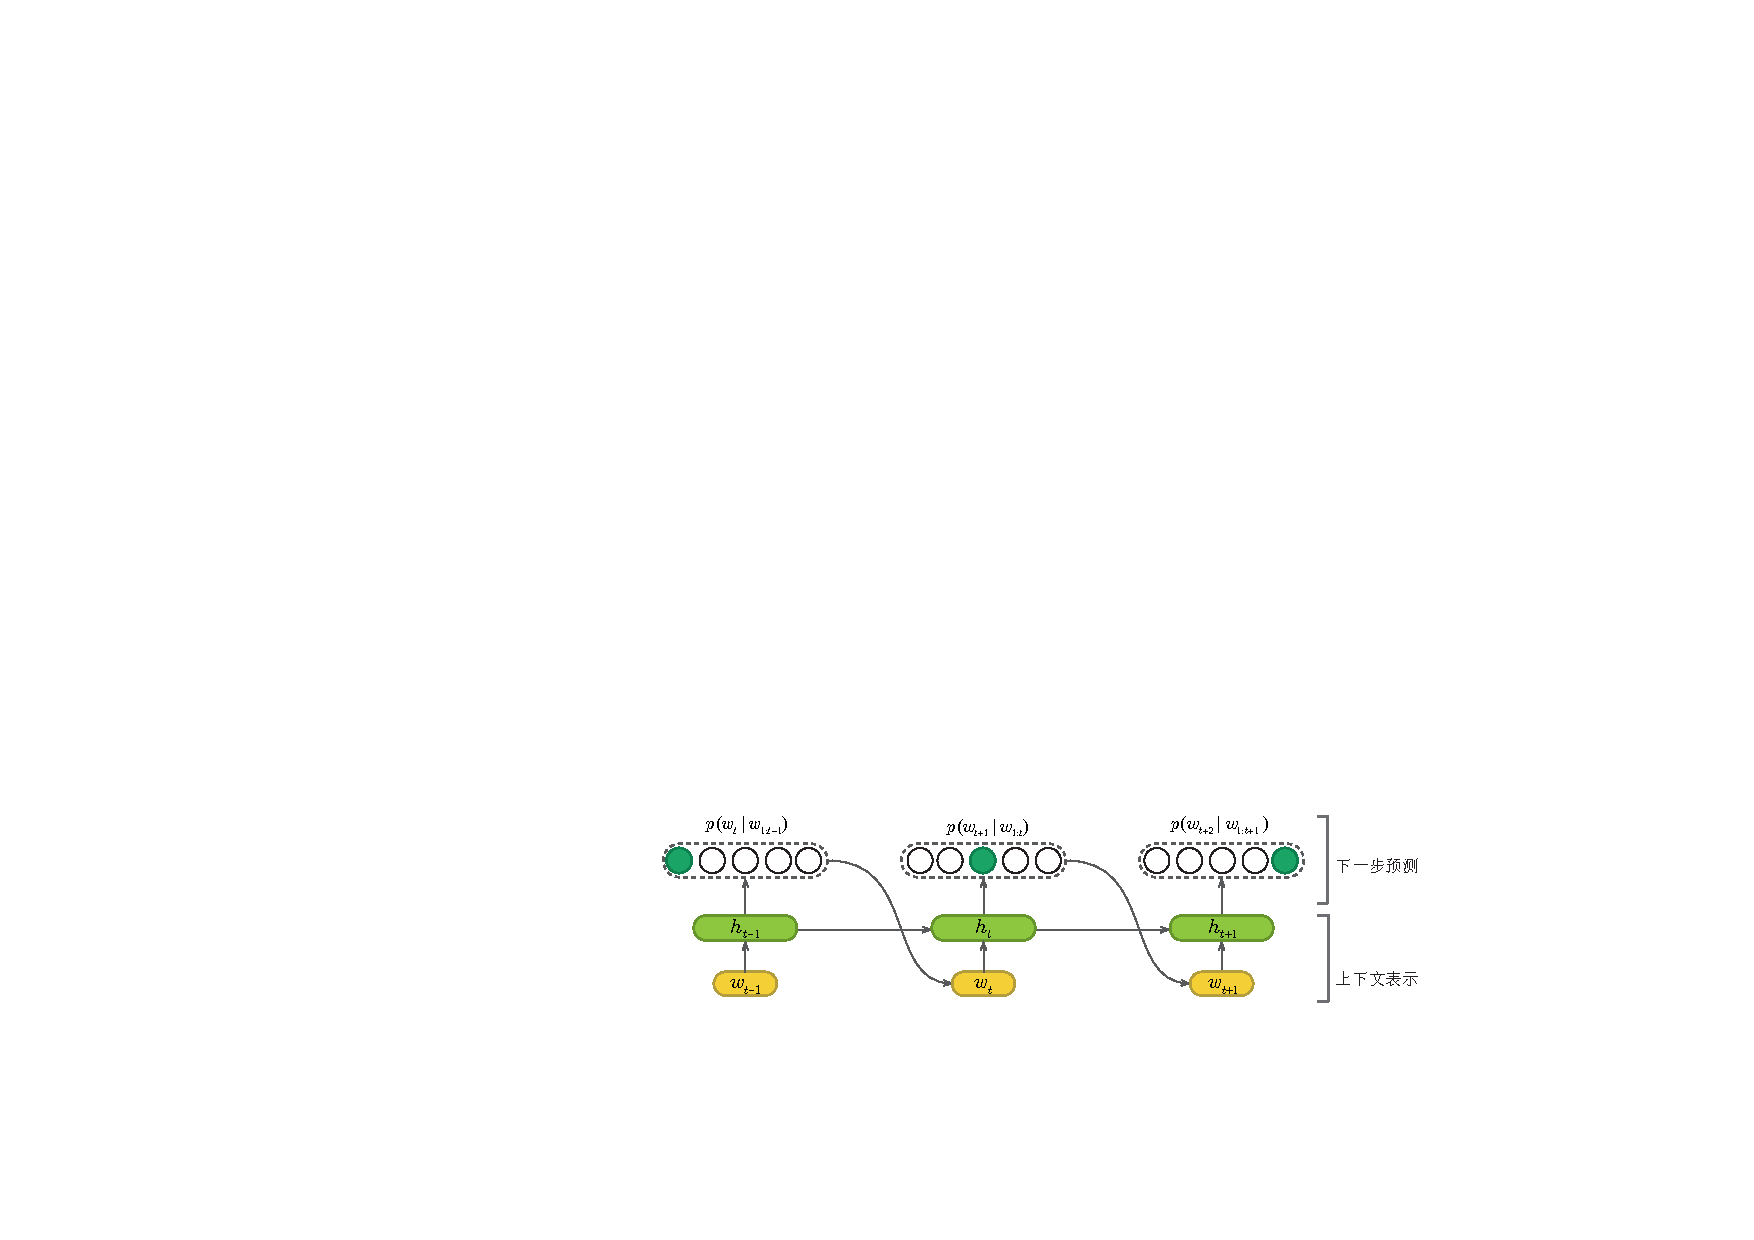
\includegraphics[width=1\columnwidth]{./figures/lm.pdf}
  \caption{循环神经网络语言模型图例}
  \label{fig:lm}
\end{figure}

\subsection{循环神经网络}
所以,考虑到上述长距离依赖问题,本实验采用的基准模型就是基于循环神经网络的语言模型。最近,利用序列的时间序列信息的循环神经网络已经非常流行,如图~\ref{fig:lm}~所示。 为了清楚起见,由于在当前时间步 $ t $的输出$ w_ {t + 1} $正好是下一个时间步的输入$ w_ {t + 1} $,所以没有输出的自动关联连接(Auto-associative Connection)的前一次步骤$ t $回到下一个时间步骤$ t + 1 $中的循环神经网络。每个句子都需要用开始词(即,$ \langle s \rangle $)和结束词(即$ \langle / s \rangle $)标记进行封装。 在预测下一个单词 $ w_ {t + 1} $ 之前,从最后一个隐藏状态$ h_ {t-1} $和当前字$ w_t $接收到循环网络单元的输入。

从形式上讲,循环神经网络是一个参数化的非线性函数$ \mathtt{RNN} $,循环地将一系列向量映射到一系列隐藏状态。 将$ \mathtt{RNN} $应用于任何这样的序列,在每个时间步骤$ t $产生隐藏状态$ h_t $,如下所示:
\begin{equation}
  h_t \leftarrow  \mathtt{RNN}(W\theta^w_t + U h_{t-1} +c),
\end{equation}
其中$ W,U $是模型参数的集合,而$ U $是随时间共享的,向量$ \theta^w_t$ 对应于源词的嵌入$ w_t $。

自Elman提出基本循环网络模型~\upcite{DBLP:journals/cogsci/Elman90}~以来,已经有许多扩展模型提出了克服长距离依赖,梯度消失(Gradient Vanishing)和梯度爆炸(Gradient Exploding)等问题, 如长期短期记忆网络(LSTM)~\upcite{7508408},门限记忆单元(GRU)~\upcite{DBLP:conf/nips/ChungKDGCB15}和近似递归神经网络(Quasi-RNNs)\upcite{DBLP:journals/corr/BradburyMXS16}。

\begin{figure}[!ht]
  \centering
  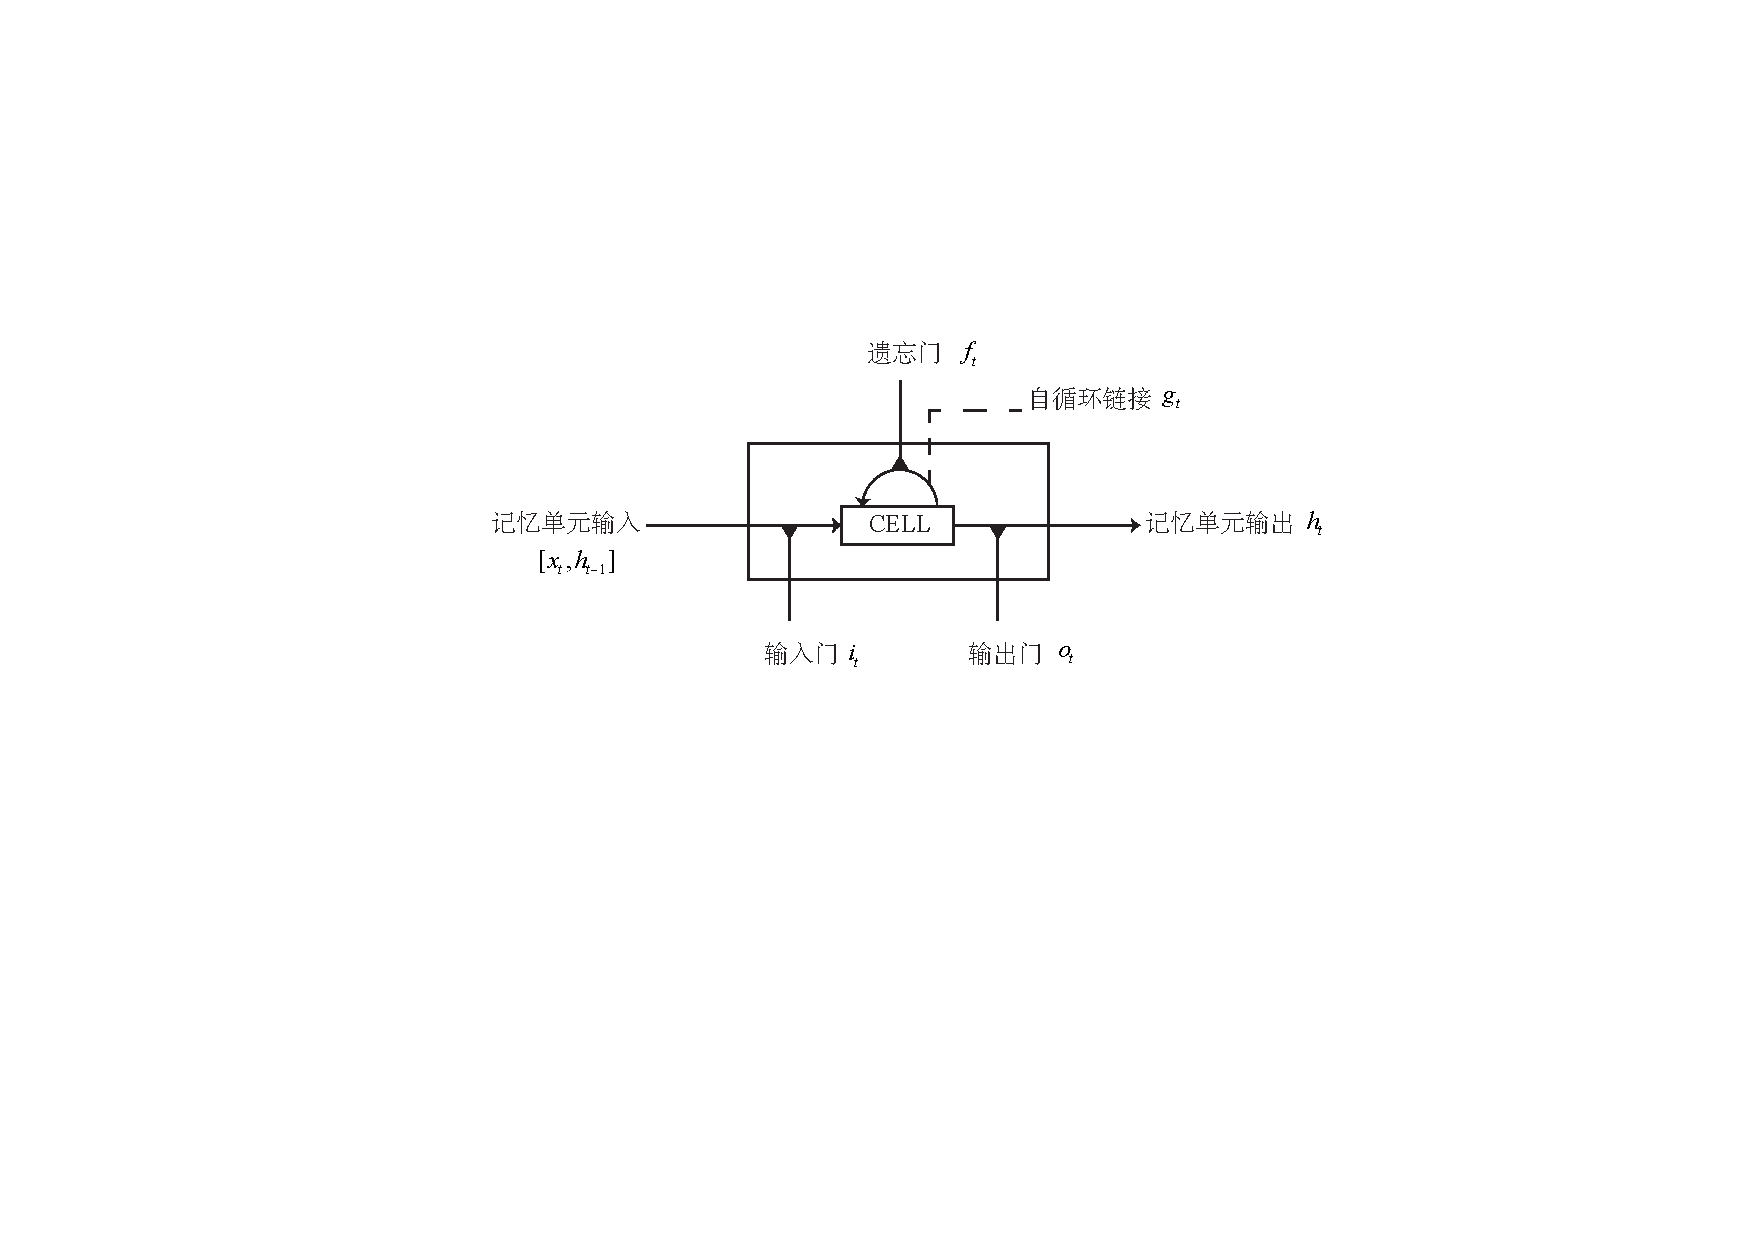
\includegraphics[width=0.7\linewidth]{./figures/lstm.pdf}
  \caption{LSTM 模型示意图}\label{fig:lstm}
\end{figure}

{长距离短期记忆网络}。LSTM的计算公式定于如下 \upcite{DBLP:journals/neco/HochreiterS97}:
\begin{itemize}
\item 输入门。控制当前输入 $x_t$ 和前一步输出 $h_{t−1}$ 进入新的 cell 的信息量:$i_t=\sigma(W^i x_t+U^i h_{t-1}+b^i)$
\item  遗忘门。决定是否清楚或者保持单一部分的状态$f_t=\sigma(W^f x_t+U^f h_{t-1}+b^f)$
\item  变换输出和前一状态到最新状态$g_t=\phi(W^g x_t+U^g h_{t-1}+b^g)$
\item  输出门。计算 cell 的输出$o_t=\sigma(W^o x_t+U^o h^{t-1}+b^o)$
\item  cell 状态更新。步骤:计算下一个时间戳的状态使用经过门处理的前一状态和输入:$s_t=g_t\odot i_t+s_{t-1}\odot f_t$
\item 最终 LSTM 的输出:使用一个对当前状态的 $\tanh$ 变换进行重变换:$h_t=s_t\odot \phi(o_t)$
\end{itemize}
\noindent 其中$\odot$ 代表对应元素相乘(Element-wise Matrix Multiplication), 函数 $\phi(x), \sigma(x)$ 的定义如下:
\begin{equation}\label{equ:tanh}
  \phi(x)=\frac{e^x-e^{-x}}{e^x+e^{-x}},\sigma(x)=\frac{1}{1+e^{-x}}
\end{equation}

{并行计算实现方法}。输入门、遗忘门、输出门和状态更新门矩阵乘法可以并行实现,从而提高LSTM模型的计算效率。因为LSTM的计算模型更容易并行,所以他与GRU的计算时间相差无几,尽管LSTM的模型需要的参数量是GRU模型的1.5倍。
\begin{equation}\label{equ:lstm}
\begin{bmatrix} i^t\\ f^t\\g^t\\o^t \end{bmatrix} =\begin{bmatrix}\sigma\\ \sigma\\\phi\\\sigma\end{bmatrix}\times W\times[x_t,h_{t-1}]
\end{equation}
其中 $W$ 指的是四个小矩阵互相层叠起来 $[W^i,W^f,W^g,W^o]$。




{门限记忆单元。} GRU 可以看成是 LSTM 的变种,GRU 把 LSTM中的 遗忘门和输入门用更新门来替代。 把 cell state 和隐状态 $h_t$ 进行合并,在计算当前时刻新信息的方法和 LSTM 有所不同。 下图是GRU更新 $h_t$ 的过程\upcite{DBLP:journals/corr/Pezeshki15}, 具体定义如下:
\begin{figure}[!h]
  \centering
  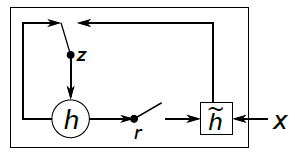
\includegraphics[width=0.45\linewidth]{./figures/gru.png}
  \caption{GRU模型示意图}\label{fig:gru}
\end{figure}

\begin{itemize}
\item 更新门 $z_t$。定义保存多少以前的信息: $z_t = \sigma ( W^z x_t+ U^z h_{t-1}  )$

\item 重置门 $r_t$。 决定保留多少输入信息: $r_t = \sigma(W^r x_t  + U^r h_{t-1}  )$

\item 节点内部更新值$\tilde h_t $。 其次是计算候选隐藏层(candidate hidden layer) $\tilde h_t$,这个候选隐藏层 和LSTM中的$\tilde c_t$是类似,可以看成是当前时刻的新信息,其中$r_t$用来控制需要 保留多少之前的记忆,如果$r_t$为0,那么$\tilde h_t$只包含当前词的信息:$\tilde h_t  = \tanh (W^h x_t  + U^h(h_{t-1} \odot r_t) )$

\item 隐藏层输出值$h_t$。 最后$z_t$控制需要从前一时刻的隐藏层 $h_{t-1}$ 中遗忘多少信息,需要加入多少当前 时刻的隐藏层信息$\tilde h_t$,最后得到$h_t$,直接得到最后输出的隐藏层信息, 这里与LSTM的区别是GRU中没有 输出门:$h_t = (1-z_t)\odot \tilde h_t  + z_t \odot h_{t-1}$
\end{itemize}

如果重置门接近0,那么之前的隐藏层信息就会丢弃,允许模型丢弃一些和未来无关 的信息;更新门 控制当前时刻的隐藏层输出$h_t$需要保留多少之前的隐藏层信息, 若$z_t$接近1相当于我们之前把之前的隐藏层信息拷贝到当前时刻,可以学习长距离依赖。 一般来说那些具有短距离依赖的单元重置门比较活跃(如果$r_t$为1,而$z_t$为$0$ 那么相当于变成了一个标准的RNN,能处理短距离依赖),具有长距离依赖的单元更新门比较活跃。



\section{大词表问题}
作为多标签分类(Multi-class Classification)的标准概率归一化方法,对于大词表问题中,\texttt{log-softmax} 函数和相应的梯度(Gradient)可以定义为:
\begin{equation}
\begin{split}
p(w|h)=&\frac{\exp(h^\top v_{w})}{\sum_{w_j\in \mathcal{V}}{\exp(h^\top v_{w_j} )}} \\
\frac{\partial p(w_i|h)}{\partial v_{w_j}}=&p(w_j|h)(\delta_{ij}-p(w_i|h))h^\top\\
\end{split}
\end{equation}
\begin{equation}
\label{eq:softmax}
\begin{split}
\log p(w|h) &= \theta^w h-\log \sum_{u\in \mathcal{V}}{\exp(\theta^u h)}\\
\nabla_{\theta^u}{\log p(w|h)}&= (\delta_{uw}-p(w|h))h
\end{split}
\end{equation}
其中$ h $是隐藏层输出的向量(即上下文表示),$ \theta ^ w $表示单词$ w $的目标单词嵌入~\upcite{duda2012pattern}。 同样对于克罗内克 $\delta$ 函数$ \delta_ {uv} $(Kronecker Function),如果$ u,v $指代的是相同的单词结果是$ 1 $,如果$ u,v $指代的不是相同的单词则是$ 0 $。


如等式~\ref{eq:softmax}~所示,前向概率传播函数$\log p(w|h) $(即第一行方程)和后向梯度优化函数$\nabla_{\theta^u}{\log p(w|h)}$(即第二行的方程)都需要计算目标词汇表中的所有单词,因此在这个部分上花费的时间会随着词表中包含的单词数量的增加而线性增长。对于包含$ \mathcal{| V |} $ 数量的单词来说,总的时间复杂度是$ \mathcal {O}(\mathcal {| H || V |})$,其中$ \mathcal {| H |} $表示隐藏层输出的维度。即使对于采用现代通用计算体系结构的GPGPU来说, 尽管其非常适合于具有高计算并行的矩阵乘法,这种计算负担也是相当高的。因此,采用现代硬件体系结构的训练和推理中,输出字嵌入矩阵的超大尺寸仍然是一个计算瓶颈。而且,目前的设备的显存是有限的,不能任意增大显存大小,所以对词表大小有一个天然的上限。

值得注意的是,\texttt{softmax} 算法的瓶颈不能归因于``for''循环函数(即方程~\ref{eq:softmax}~)中的$ \sum_ {u \in \mathcal {V}} $,尽管它随着词汇量的增长而线性增长,但是矩阵张量的乘法计算的规模较大。因为矩阵计算需要更多的时间来获得结果,但线性求和可以更快地计算完成。所以,相比于``for''循环函数而言,主要的计算时间用于矩阵乘法计算。我们在这里说明的目的是,只有那些避免其他冗余字的计算概率才能达到边际加速比的方法,而那些仍然涉及全局概率规一化的方法,实际上并不能真正改善这个部分的计算占用的时间。

%其中由于分母是正则项,一旦词表扩大,每次迭代更新都需要计算这一项,是主要的问题所在,所以本课题拟在主要解决该问题所导致的计算费时的问题,

因此,在保证计算精度不下降的情况下,我们期望能缓解计算概率归一化项的计算瓶颈并且提高模型的训练速度。 目前主要缓解大词表问题的算法主要分为以下三类: 单词拆分算法(Vocabulary Truncation)、采样估计模型(Sampling-based Approximation)和层次分解模型(Vocabulary Factorisation)。下面我们将一一详述。


\subsection{单词拆分算法}
针对大词表问题的解决方法,最直接最简单的策略就是我们放弃使用大词表,转而保留一个较小的词表来保证训练的内存占用小和计算效率高。那么针对剩余的过多的词表外的单词(Out-Of-Vocabulary,OOV),我们可以使用传统的N-gram语言模型来估算其可能的概率分布。这样做一方面保证神经网络模型可以在有限时间内训练完,同时保证模型的最后的测试结果不会很差~\upcite{DBLP:journals/csl/Schwenk07}。

然而我们需要注意到,当我们的词表继续减少和我们的所有单词种类不断变多的时候,我们会发现训练样本中存在过多的$\langle$unk$\rangle$ 字符,这样使得神经网络的模型训练非常困难,进而导致模型效果变得非常地差,所以这种方案只是一定程度上缓解了大词表问题,但是也是一种有效的尝试方案。

除了上述直接的建模方案外,目前采用的方案是将单词按照字符级别来划分,可以将一个单词按照字符统计规律划分成任意多个子词。其中二元对编码(byte-pair-encoding,BPE)能将一个单词划分成两部分:前缀(Prefix)和后缀(Suffix)~\upcite{DBLP:conf/icassp/Tucker0P94, DBLP:conf/acl/SennrichHB16a,Gage:1994:NAD:177910.177914},如图~\ref{fig:subword} 所示。从该图中我们可以看出,单词被划分成前缀和后缀两部分,其中$+$代表是单词的前缀,同时$\langle /w \rangle$是单词的后缀。由于划分规则是从训练数据中学习到的,我们可以指定需要缩减的词表大小,所以该算法的动态适应性很强,目前主流的机器翻译模型都采用这个方案~\upcite{DBLP:journals/corr/JozefowiczVSSW16}。尽管如此,我们仍然需要看到它这样的解构操作依然带来了一定的损失,因为句子的长度加倍了,对RNN的长距离关系学习能力提出了更高的挑战~\upcite{DBLP:conf/aaai/KimJSR16}。

\begin{figure}[!h]
  \centering
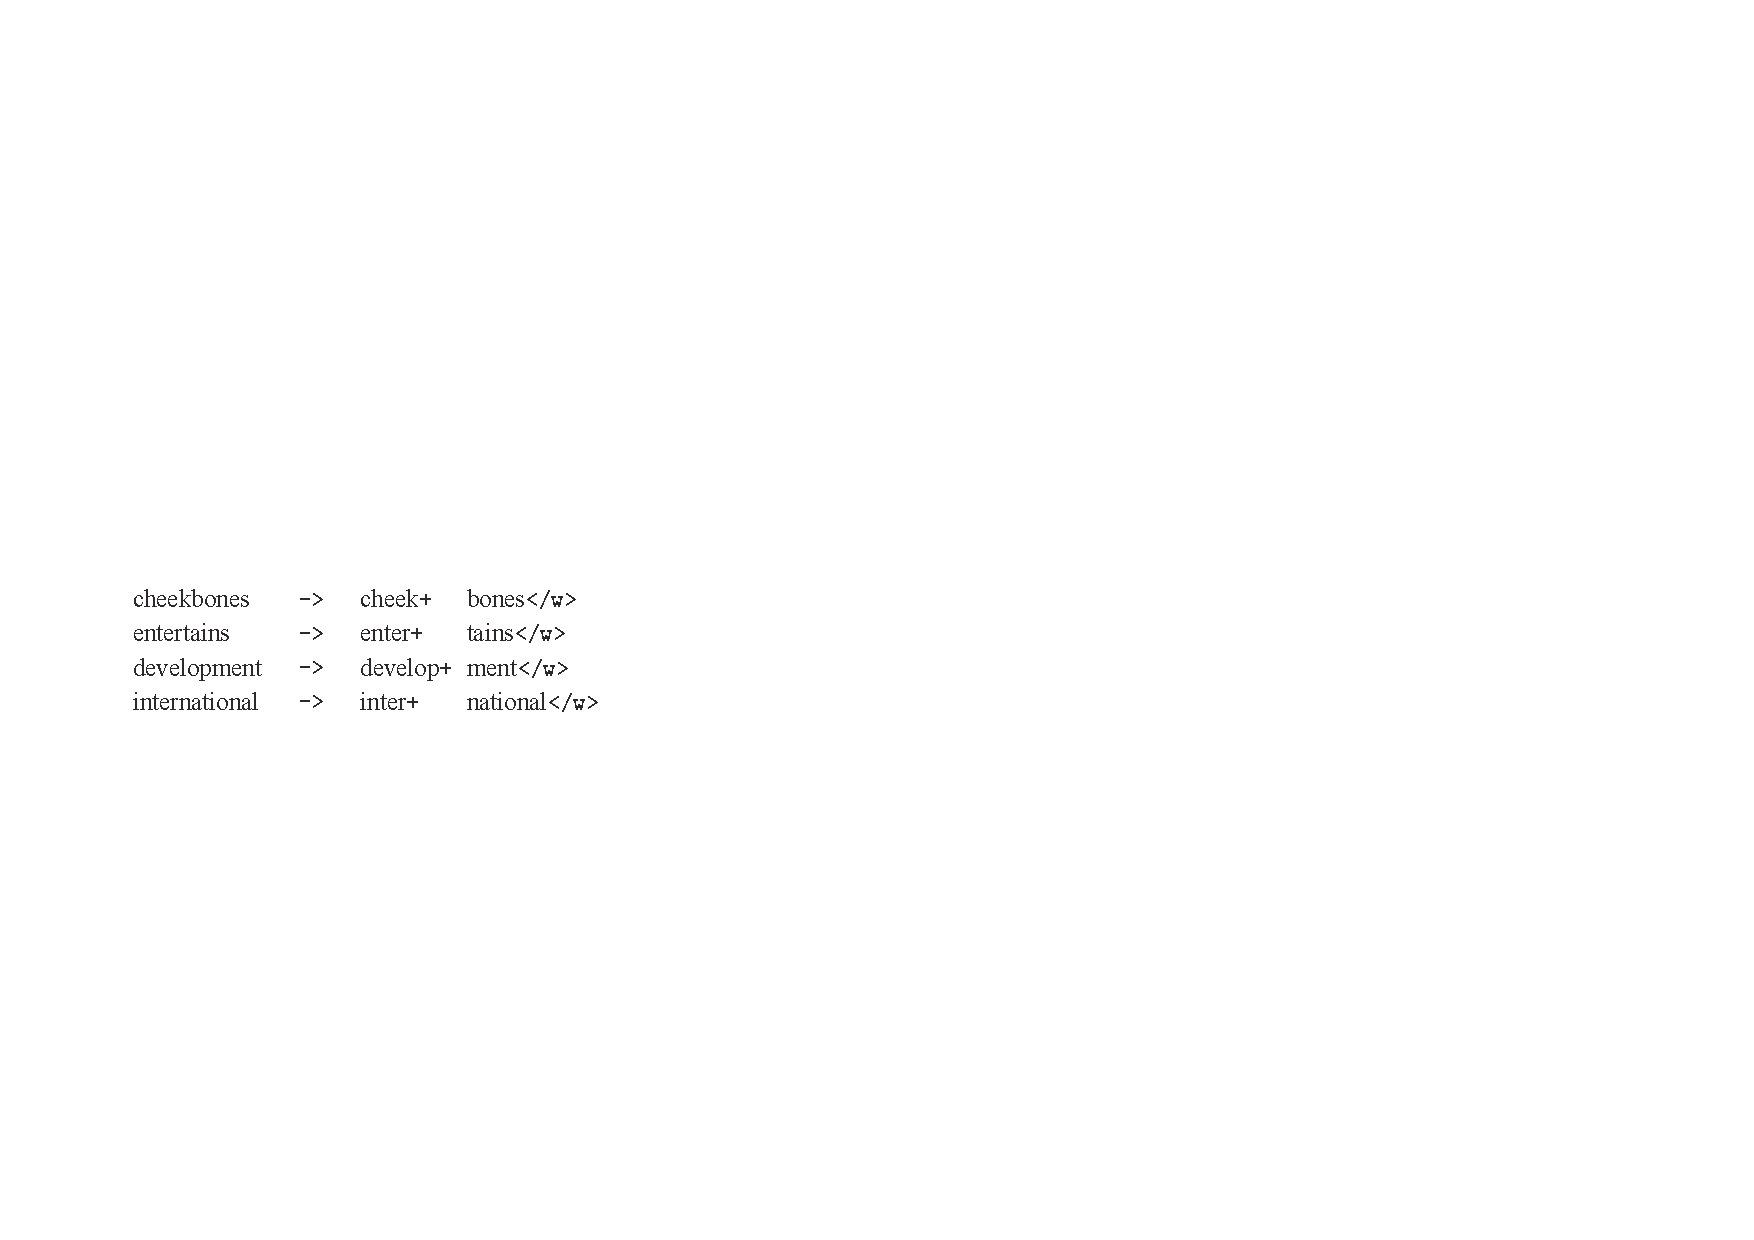
\includegraphics[width=0.6\linewidth]{./figures/subword.pdf}
\caption{词到子词划分样例}\label{fig:subword}
\end{figure}

\subsection{采样估计模型}
目前采用的采样算法(Sampling Algorithm)主要是针对公式~\ref{eq:softmax}~中对所有单词概率规约那一项进行概率估计,其中著名的算法有:重要性采样(Importance Sampling)~\upcite{DBLP:journals/tnn/BengioS08},噪声差分估计(Noise Contrastive Estimation, NCE)~\upcite{DBLP:conf/icml/MnihT12}和Blackout 采样算法~\upcite{DBLP:journals/iclr/JiVSAD15}。第一种算法在Bengio的实验中被证明模型无法收敛~\upcite{DBLP:journals/tnn/BengioS08},因此目前主要使用的后面两种算法。

对于NCE噪声差分估计算法来说,模型需要学习将正确的单词 $w_0$ 与随机生成的单词 $\{w_1\cdots w_k\}$做一个二元分类。 其中 $w_0$ 训练样本中真正的下一个单词, $\{w_1\cdots w_k\}$ 是采用先验分布  $q(w)$产生的随机噪声单词. 正例归一化后的概率和所有负例联合概率的公式可以写成:
\begin{equation}\label{equ:nce}
\begin{split}
  \tilde{p}(y=1|h)=&\frac{\exp( \theta^w_0 h)}{ \exp( \theta^w_0 h)+k *q(w_0)}\\
  \tilde{p}(y=0|h)=&\prod_{i=1}^{k}\frac{k *q(w_i)}{\exp( \theta^w_i h)+k *q(w_i)}\\
\end{split}
\end{equation}
需要注意的是噪声概率 $\tilde{p}(y=0|h)$ 需要对 $k$ 个噪声样本做加法运算而不是对整个词表单词进行的。 这样的话该算法的计算机复杂度就是$\mathcal{O}(k+1)$,和整个词表的大小无关了。从而该算法的加速比是$\mathcal{O}(\mathcal{|V|}/(k+1))$

除此之外,最近提出的Blackout采样算法针对噪声概率归一化的时候与当前上下文的相关,对上述的NCE算法进行了进一步优化和修正~\upcite{DBLP:journals/iclr/JiVSAD15},同时也引入了更多的计算量。其模型的代价函数计算公式定义为:
\begin{equation}
\begin{split}
  \ell=&-\log(p(w_0|h)) - \sum_{w_i \sim p(w)} \log(1 - p(w_i))\\
p(w_i) =& \frac{\exp(\theta^w_i h)}{\sum_{w_i \sim p(w)} \exp(\theta^w_i h)}.
\end{split}
\end{equation}

总的来说,这些采样近似算法可以显着加快训练速度,但仍然需要时间来利用单词分布$q(w)$~\upcite{DBLP:conf/naacl/ZophVMK16}来采样大量的噪音单词,采样单词足够多的情况占用的时间仍然很客观,需要进一步手段优化。 另一方面,Softmax函数在推理测试的时候必须要计算,意味着在测试推理的时候该算法失效了。因为候选词是在整个词汇表中预测的,而不仅仅对当前的采样的早噪声单词做预测,而且我们更无法得知正确的单词是什么\upcite{DBLP:journals/jmlr/GutmannH12}。

这里我们需要注意的是,由于我们引入了采样函数$q(w)$,模型会花费额外时间在采样计算上面。从离散分布采样的初始程序通常需要词汇数量具有线性时间复杂度。因此我们需要寻找一个性能优异的带权重的随机数生成器或者是离散采样函数。


\subsection{层次分解模型}
层次分解方法,可以大大降低学习和推理过程中表示概率分布的所占用的计算内存,因为它只计算局部概率并且选择每一层的分数最高的候选路径而不是保存全局计算结果。
目前主要的分解策略可以分为: 基于类别的多元分类模型(class-based hierarchical softmax, cHSM)和基于二叉树的二元分类模型(class-based hierarchical softmax, tHSM)。接下来我们将这两种算法的详细计算过程进行描述。

首先我们考虑基于类别的分解策略。假设语料中的每一个词样本属于且只属于一个类(class或者group),在此基础上计算词样本在语料中的分布时,可以先计算类的概率分布,然后在所属类上计算当前词的概率分布,于是可将公式~\ref{eq:softmax} 转化为:
  \begin{equation}
  \begin{split}
p(w|h)=&p^c(\mathcal{C}(w)|h)\cdot p^w(w|\mathcal{C}(w),h) , w\in \mathcal{C}(w),\\
&\mathcal{V}=\bigcup _{i = 1}^\mathcal{C}{c_i},\quad  c_i \bigcap c_j=\phi, \text{若}\quad i\ne j, \\
\end{split}
\end{equation}
其中 概率~$p^c(\mathcal{C}(w)|h)$~表示每个类别的概率,$p^w(w|\mathcal{C}(w),h)$~表示在类别$\mathcal{C}(w)$中所有单词的局部概率。

此时,训练一个词样本的计算复杂度正比于: $\mathcal{O =|H||C|}$。 在该计算公式中,$\mathcal{C}$ 为语料中所有词的分类数,可根据语料中词的词频进行划分。 当$C$ 取$1$ 或取词典大小$|V|$ 时,此结构等同于标准的Softmax 结构,此时词表还是原来的结构,并没有任何优化效果。因此,对于绝大多数情况,我们取$\mathcal{C} \ll \mathcal{V}$并且 $|\mathcal{C}|\ll 1$,这样的结构才能保证有效降低 softmax 的计算复杂度。图~\ref{fig:case_hsm} 展示了类别划分和分步概率计算的示例。从图中我们可以得知,其中词表 [duck,cat,mop,broom] 被划分成两个类别:$c_1\to$[duck,cat],$c_2\to$[mop,broom]并且$c_3\to$[the,am]。
\begin{figure}[!h]
  \centering
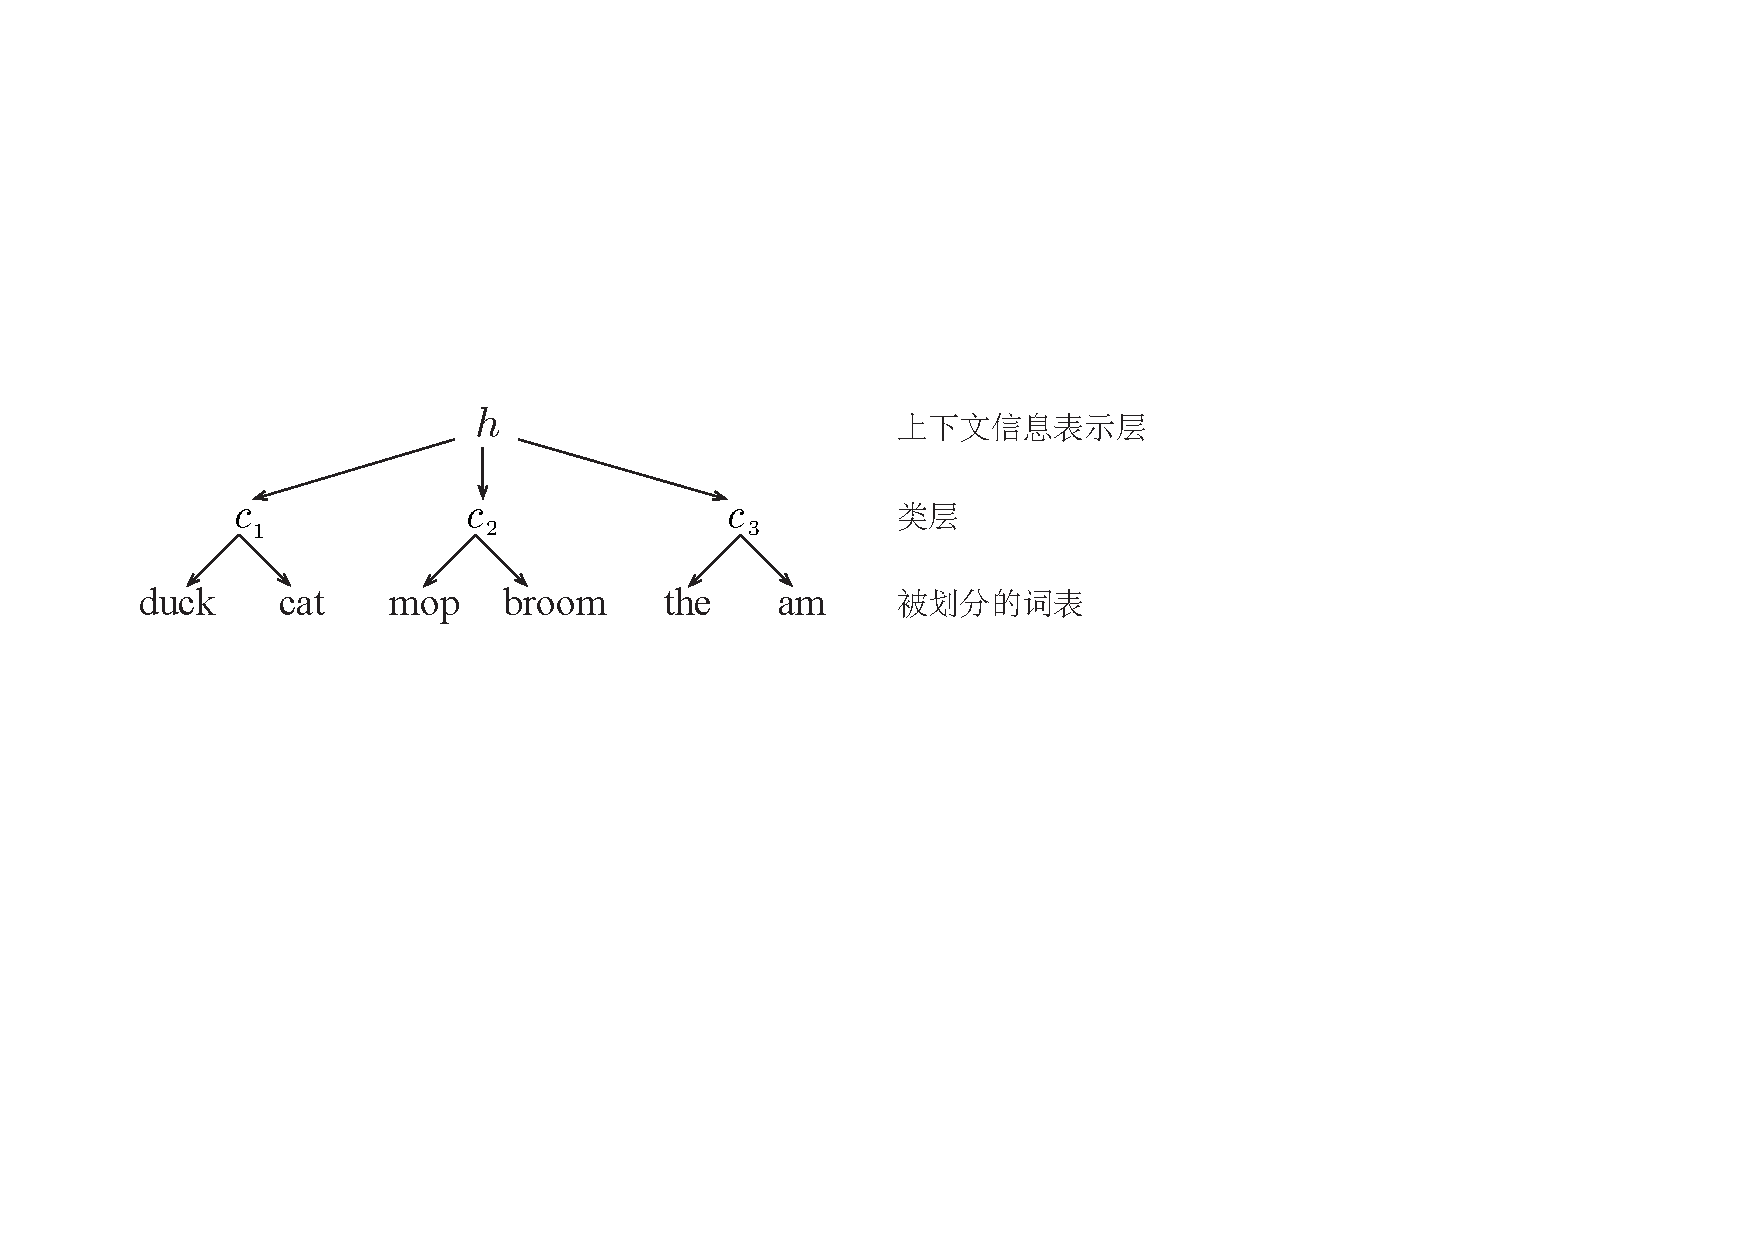
\includegraphics[width=0.79\linewidth]{./figures/case_chsm.pdf}
\caption{cHSM算法可视化模型}\label{fig:case_hsm}
\end{figure}

假设每个类包含 $\sqrt{\mathcal{|V|}}$ 单词,表示词汇被划分为相同大小的组,这样的话级联概率(cascaded probability)只涉及$2\sqrt{\mathcal{|V|}}$ 单词 softmax计算,所以最优时间复杂度可以减少到$\mathcal{O}(\mathcal{|H|}\sqrt{\mathcal{|V|}})$~\upcite{DBLP:conf/icassp/Goodman01}。虽然在更常见的情况下,分区算法会产生不同大小的字组,这需要外部的其他结构来建立高效的数据结构,并且这些稍微复杂的算法尚未被完全探索和分析。此外,我们还可以通过不同的类大小和分区算法来调整精度和效率之间的权衡关系。

另一方面,我们再介绍基于二叉树分解词表的建模策略。tHSM方法将一步多类分类分解为多个二元分类步骤。正因为如此,词汇组织为二叉树,其中单词分布在二叉树的叶子节点上,二叉树的所有的中间节点的都是内部参数。如果该二叉树是平衡树的结构情况下,每个词将会被赋予相等长度的前缀,最优时间复杂度可以减少到$\mathcal{O(|H|\log \mathcal{|V|})}$。最早的工作中,单词在二叉树上的分布可以由WordNet与人类专家~\upcite{DBLP:conf/aistats/MorinB05}或单词 unigram 分布~\upcite{DBLP:conf/nips/MikolovSCCD13}的霍夫曼编码构建。然而,在现实世界的大规模文本应用中,专家知识的构建是相当昂贵的。所以,一般人们也不会采用这样的方案来构建单词的二叉树分布。霍夫曼编码方案只考虑单数据统计,而单词的语境,句法或语义信息尚未被考虑和得到彻底的讨论。

\begin{figure}[!h]
  \centering
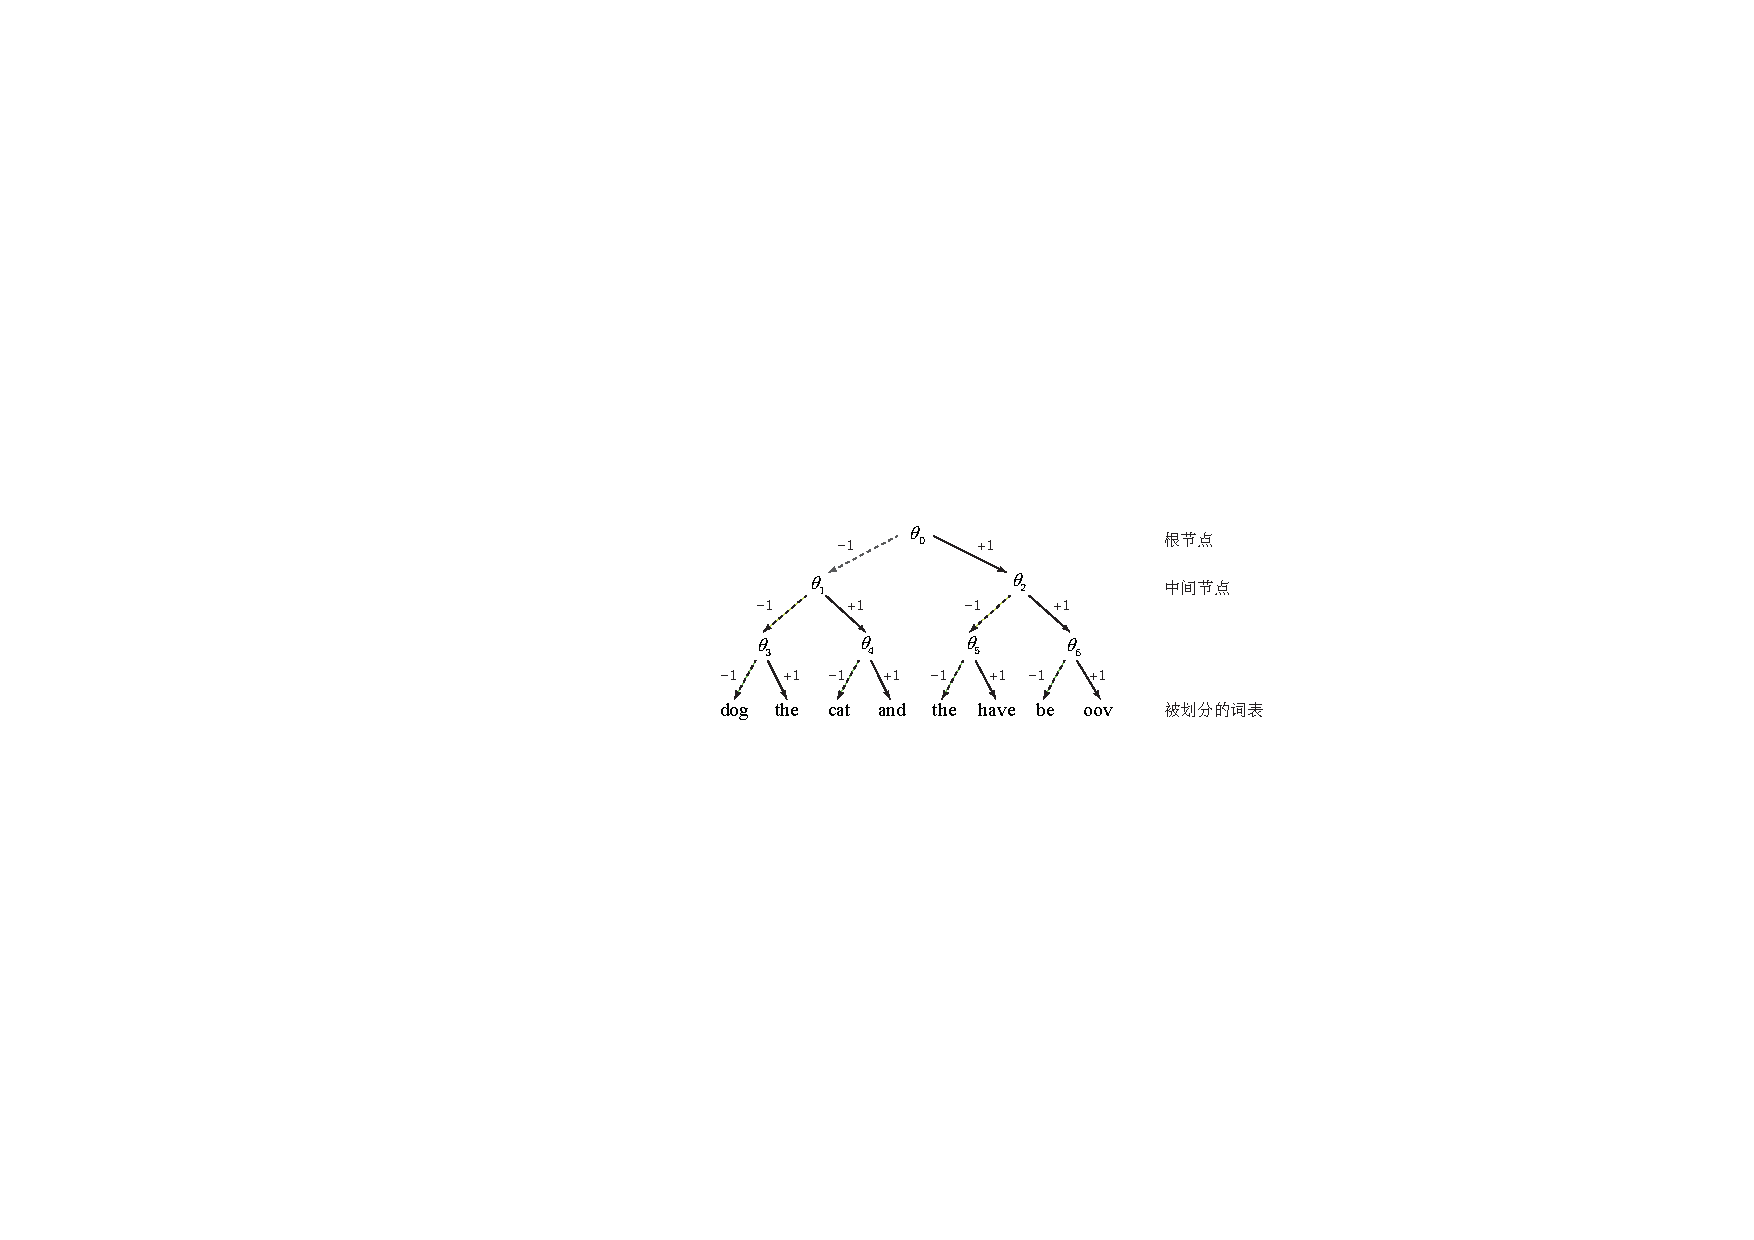
\includegraphics[width=0.9\linewidth]{./figures/thsm-example.pdf}
\caption{tHSM算法可视化模型}\label{fig:case_thsm}
\end{figure}

图~\ref{fig:case_thsm} 展示了二叉树概率分解和计算的示例。

Mikolov当年曾提出使用基于二叉树的层级softmax模型来加速的训练方案,加速比能达到理论的最大速度。但是需要注意的是,当时提出的背景是基于CPU计算方案构建的,如今随着应用领域的推广越来越多的算法应用到实际问题中,我们需要在并行度更高的GPU上进行计算,因此基于GPU进行建模的tHSM和历史上研究众多的cHSM算法尚未被研究提及,因此我们将会需要在本文中详细研讨。

\section{离散采样算法}
在我们使用基于采样的模型时,我们不可避免的需要使用到离散采样函数,即:设一共有$|\mathcal{V}|$个单词,第$i$个单词出现的概率是$p(w_i)$, 如何高效地产生这样的随机变量序列$w_1,w_2,\cdots$?

这问题其实正式来说,可称为模拟离散取样(Simulated Discrete Sampling),跟据有限类别的指定的概率,来模拟取样,生成采样序列输出。其中,要制造指定的概率分布随机变量,关键就是如何通过均匀分布变换获得。因为我们的计算机只能快速产生伪随机数,即均匀分布的采样输出。其他的复杂采样函数均建立在均匀分布的变换之上。
\subsection{随机采样函数}
当我们使用概率模型实现推理和学习算法时,通常需要从离散分布进行抽样。 也就是说,从参数$\boldsymbol {\pi} \in \mathbb{R} ^ K$中的多项式分布,使得$\ pi_k \geq 0$和$\sum_{k} \pi_k = 1$。 更常见的情况是我们在$\mathbb{R}^K$中有一个$\boldsymbol {\phi}$ ,其中$\phi_k \geq 0$,但我们不知道规范化常量。 也就是说,$\boldsymbol{\pi}$只与多项式参数$\boldsymbol {\pi}$成正比。 我们希望根据$\boldsymbol{\pi}$快速生成一个变量,给出$\boldsymbol {\pi}$,用(Matlab)代码很容易地完成某些操作:
\begin{verbatim}
cdf = cumsum(phi);
samp_k = sum(cdf < rand()*cdf(end)) + 1;
\end{verbatim}
这很好很简单,但是你会注意到它具有每个样本的设置(计算CDF)和$\mathcal {O}(K)$时间复杂度的$\mathcal {O}(K)$时间复杂度。每个样本的复杂度可能被降低到$\mathcal {O}(\log K)$,找到阈值的数据结构更好。事实证明,我们可以做得更好,得到$\mathcal {O}(K)$的抽样,而仍然是$\mathcal {O}(K)$。
\subsection{基于线性搜索的逆变换方法}
在上节中,显示了CDF的一些特性,例如CDF的范围是$[0,1]$,而且是一个单调递增的(Monotonic Increasing)函数。逆变换取样算法(Inverse Transform Sampling)就是利用了这些特性,来解决上面提出的问题。其实,逆变换取样方法并不是很复杂,我们接下来详细解释。给一个目标CDF,只要计算其逆函数(Inverse Function),就可以把均匀的随机变数转换为目标CDF:
\begin{equation}\label{equ:func}
  X=F_X^{-1}(Y)
\end{equation}

这方法能用在所有CDF(包括连续及离散的)。其数学证明可参考维基百科。

下图显示这个方法的直观解读,在Y轴范围$[0,1]$里均匀取样$(y_i)$,之后向右和CDF取交点,求交点的$X$轴位置($x_i$),$X$则是符合CDF的概率分布。这个方法用在离散的情况就更简单,只需搜寻目标的CDF,找出超过均匀取样的元素即可。
\begin{figure}[!h]
  \centering
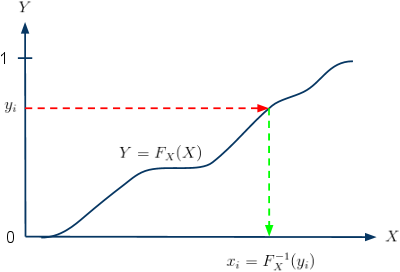
\includegraphics[width=0.5\linewidth]{./figures/cdf.png}
\caption{累计函数采样方法示意图}\label{fig:cdf}
\end{figure}
在离散的情况下(本文题目要求),其时间复杂度是O(N),其中N为类别数目。

读者可能会注意到,这里用了线性搜寻(Linear Search),如果targetPdf数组是由大至小排列,平均而言会更快找到结果。另外,也可以用二分搜寻(Binary Search),那么复杂度会降低为$O(\log |\mathcal{V}|)$,。


\subsection{基于二叉树搜索的逆变换方法}
二分搜索(binary search),也称折半搜索(half-interval search)、对数搜索(logarithmic search),是一种在有序数组中查找某一特定元素的搜索算法。搜索过程从数组的中间元素开始,如果中间元素正好是要查找的元素,则搜索过程结束;如果某一特定元素大于或者小于中间元素,则在数组大于或小于中间元素的那一半中查找,而且跟开始一样从中间元素开始比较。如果在某一步骤数组为空,则代表找不到。这种搜索算法每一次比较都使搜索范围缩小一半。

事实上,这个问题用二分搜寻是标准的方法。那么,还有没有更快的方法呢?答案是肯定的,例如别名方法(alias method)、近似方法等~\upcite{DBLP:journals/cgf/ClineRW09}。当然,在N很小的情况下,线性搜寻和二分搜寻也足够。
\subsection{别名方法}

设$ Z $为离散的随机变量,它有n个可能的结果$ z_0,z_1,\ldots,z_ {n-1} $。 为了简化下面的讨论,我们研究另一个变量$ Y $,其中$ P \{Y = i \} = P \{Z = z_i \} $。 当$ Y $取值$ i $时,让$ Z $为$ z_i $。 所以$ Z $可以从$ Y $生成。随机变量$ X $被均匀分布在$(0,n)$中,这个概率密度函数是
\begin{equation}\label{equ:alias}
 f(x) = \left\{
 \begin{array}{rl}
  1/n & \text{若 } 0 < x < n\\
  0 & \text{否则}\\
 \end{array} \right.
\end{equation}
那么我们现在生成的$Y'$是:
\begin{equation}\label{equ:gen}
  Y' =  \left\{
 \begin{array}{rl}
  \lfloor x  \rfloor & \text{若 } (x - \lfloor x \rfloor) < F(\lfloor x \rfloor)\\
  A(\lfloor x \rfloor)  & \text{否则}\\
 \end{array} \right.
\end{equation}
其中$ A(i)$是别名函数。 当$ x $落入范围$ [i,i + 1)$($ i $是一个整数)时,$ y $的概率$ F(i)$为$ i $,概率$ 1 - F(i )$是$ A(i)$。 由于$ x $是均匀分布的,
\begin{equation}
  \begin{split}
P\{x \in [i, i + F(i))\}     &= \int_i^{i+F(i)}\frac{1}{n}dx= (i + F(i) - i) \times 1/n= F(i)/n,\\
P\{x \in [i + F(i), i + 1)\} &= \int_{i+F(i)}^{i+1}\frac{1}{n}dx= (i + 1 - (i + F(i))) \times 1/n= (1-F(i))/n
\end{split}
\end{equation}

让我们将满足$ A(j)= i $的值集合$ j $表示为$ A ^ { - 1}(i)$。 生成的变量$ Y'$具有以下概率质量函数:
\begin{equation}
  P\{Y' = i\} = F(i)/n + \sum_{j \in A^{-1}(i)}\frac{1-F(j)}{n}
\end{equation}
Alias方法是构造$ A $和$ F $的算法,所以$ P \{Y'= i \} $等于$ P\{Y = i \} $。 由于$ A $和$ F $的域都是整数$ 0,1,\ldots, n-1 $,所以它们可以存储在数组中,并且可以在$O(1)$中查找值,其中空间效率是 $\mathcal{O}(n)$。

虽然别名方法可用于生成丰富的噪声字,因为它需要线性建立时间和恒定的采样时间~\upcite{10.2307/2683739,DBLP:conf/emnlp/VaswaniZFC13}。

大词表问题,主要是对softmax如何建模的问题。在本课题中,我们探讨 cHSM 和 tHSM 两种不同的方案所带来的影响和优劣。
\section{本章小结}
本章对国内外学者在语言模型的任务上相关工作进行了介绍。首先,介绍了语言模型的建模策略和对应的应用方案。并详细讨论了循环神经网络的语言模型的建模方式,并讨论了其结构的优缺点。同时为了解决使用循环网络所带来的梯度爆炸的问题,我们进而引入了长距离短期神经网络和门限记忆节点两种基于门限机制的循环网络;另一方面,我们还考虑了语言模型大规模应用所带来的大词表问题,并作了详细分析其原因。为了解决该问题,我们还讨论了历史上所提出的方案,并做了分类讨论。主要涉及三种思路:缩减词表大小,用采样算法近似估计和模型层次分解。针对各种模型提出的结果做了详细介绍,并分析了各种算法的优劣处。最后我们分析了实验中需要用到的高效采样函数的构造算法。